\section{Shuffle Test}
\label{app-shuf}
\autoref{app-shuf} contains the geometry cross sections, fission rate/thermal flux meshes, and image difference results from the shuffling tests (see \autoref{meth-sens}, Table \ref{table:shuffle}), which were omitted from the main report for brevity.

Comparing the image difference results of \autoref{app-shuf}, the shuffling test, to \autoref{app-sym}, the symmetry test, shows that the shuffling tests have a weaker effect on the fission rate and thermal flux than the symmetry tests.  The small differences in this particular test would most likely indicate that the core is generally well-mixed, i.e., that each bin in the vertical direction, along the z axis, has each of the 7 fuel compositions represented equally.


\begin{figure}[H]
\centering

\begin{subfigure}{0.45\textwidth}
  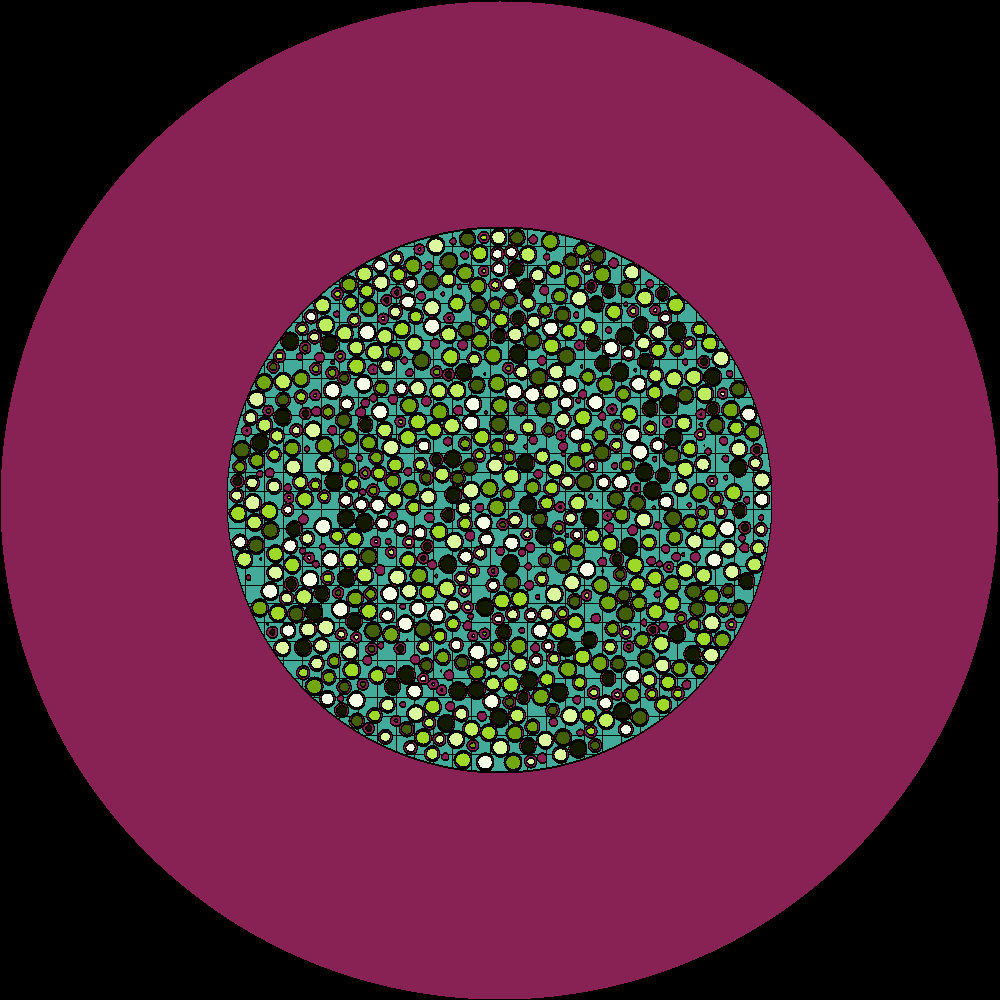
\includegraphics[width=0.95\linewidth]{figures/1234560/1234560-r}
  \caption{Radial Cross Section at y=0}
  \label{fig:1234560-r}
\end{subfigure}%
%
\begin{subfigure}{0.45\textwidth}
  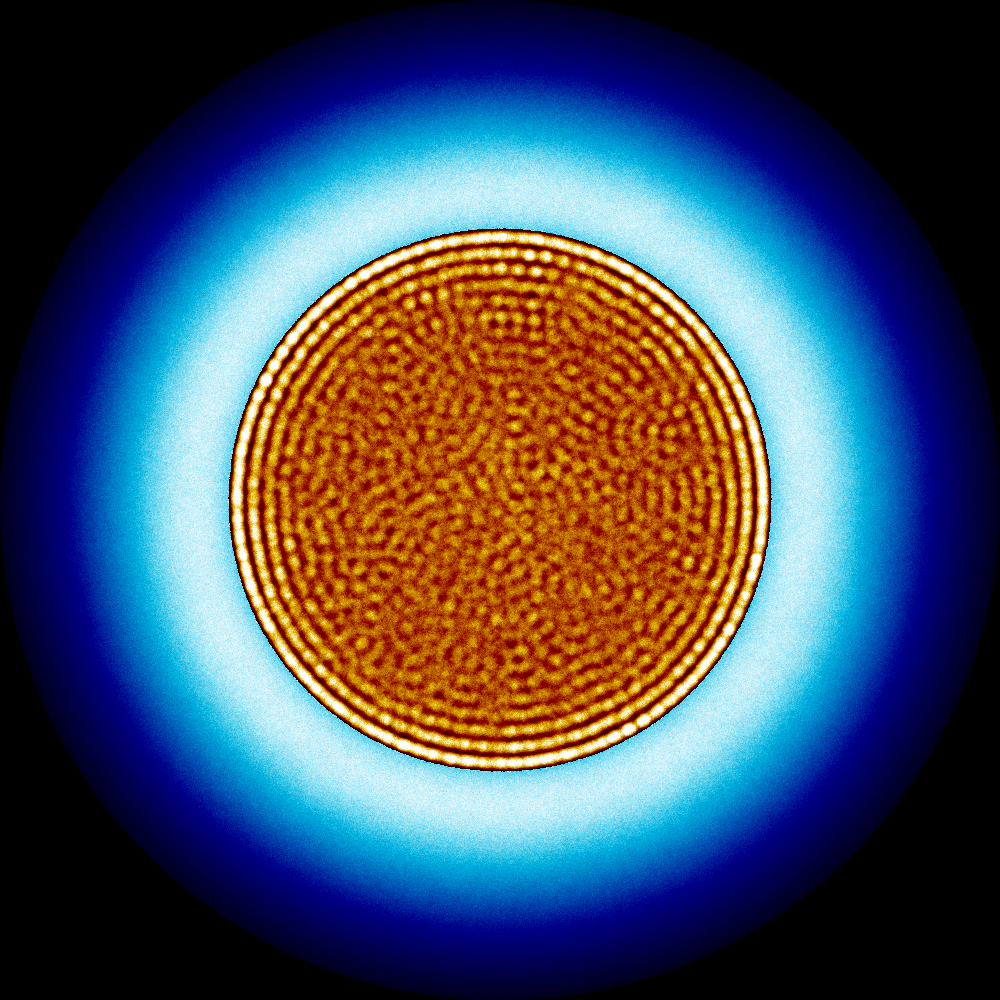
\includegraphics[width=0.95\linewidth]{figures/1234560/1234560-rm}
  \caption{Radial Mesh}
  \label{fig:1234560-rm}
\end{subfigure}

\begin{subfigure}{0.45\textwidth}
  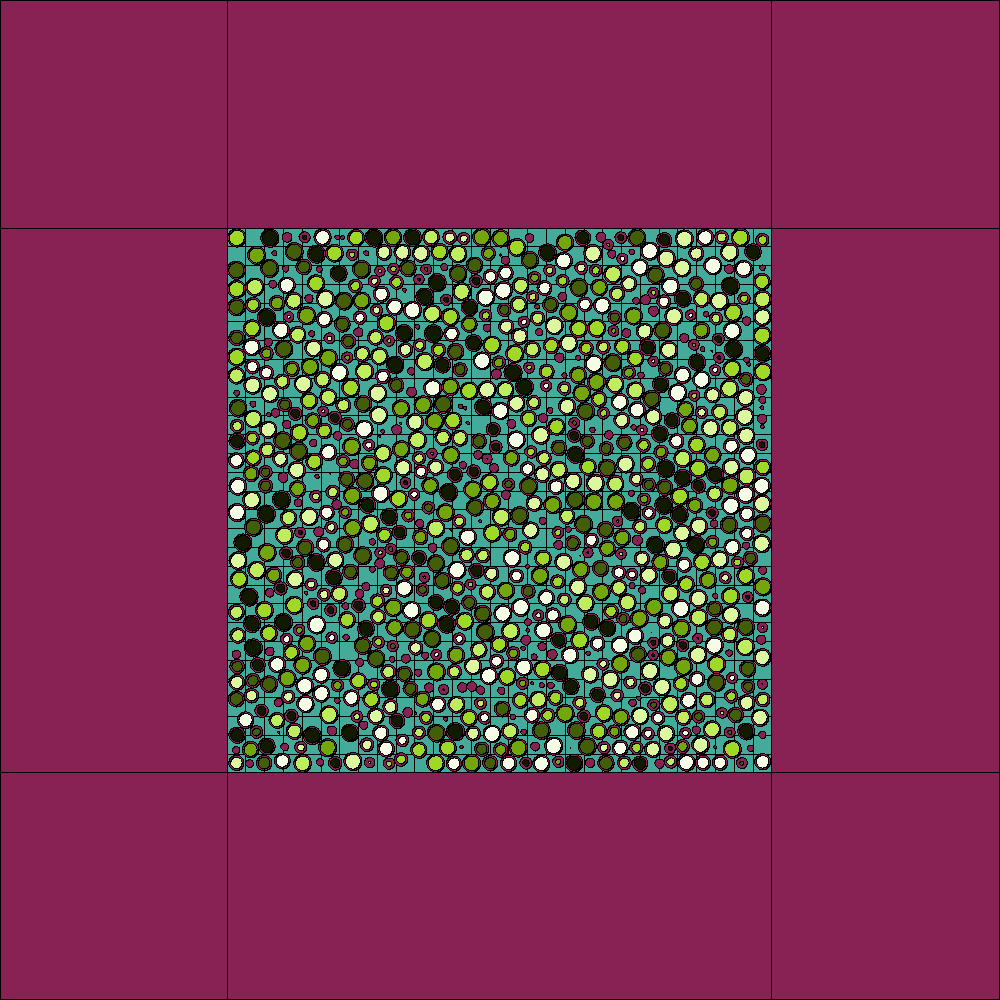
\includegraphics[width=0.95\linewidth]{figures/1234560/1234560-v}
  \caption{Axial Cross Section at z=0 }
  \label{fig:1234560-v}
\end{subfigure}
%
\begin{subfigure}{0.45\textwidth}
  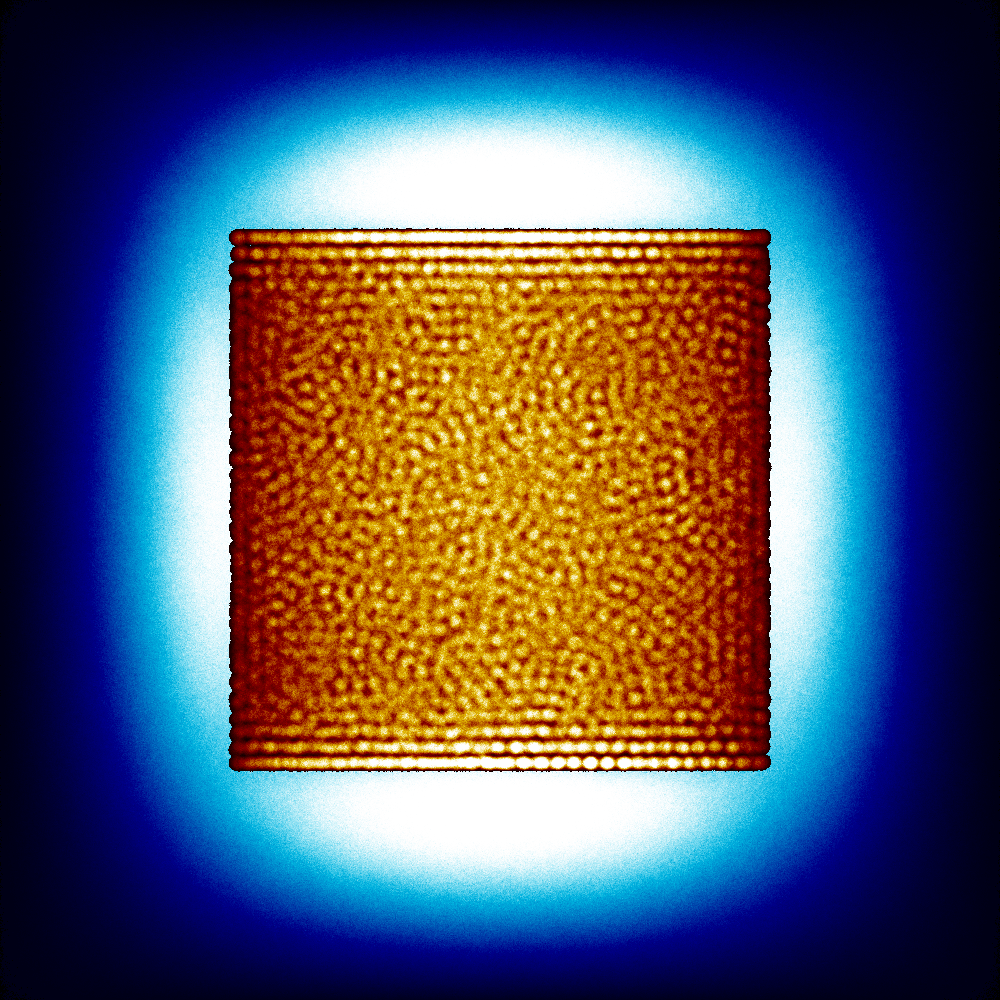
\includegraphics[width=0.95\linewidth]{figures/1234560/1234560-vm}
  \caption{Axial Mesh}
  \label{fig:1234560-vm}
\end{subfigure}
%
\caption{Shuffle Analysis: Run 1}
\label{fig:1234560}
\end{figure}
\begin{figure}[H]
\centering
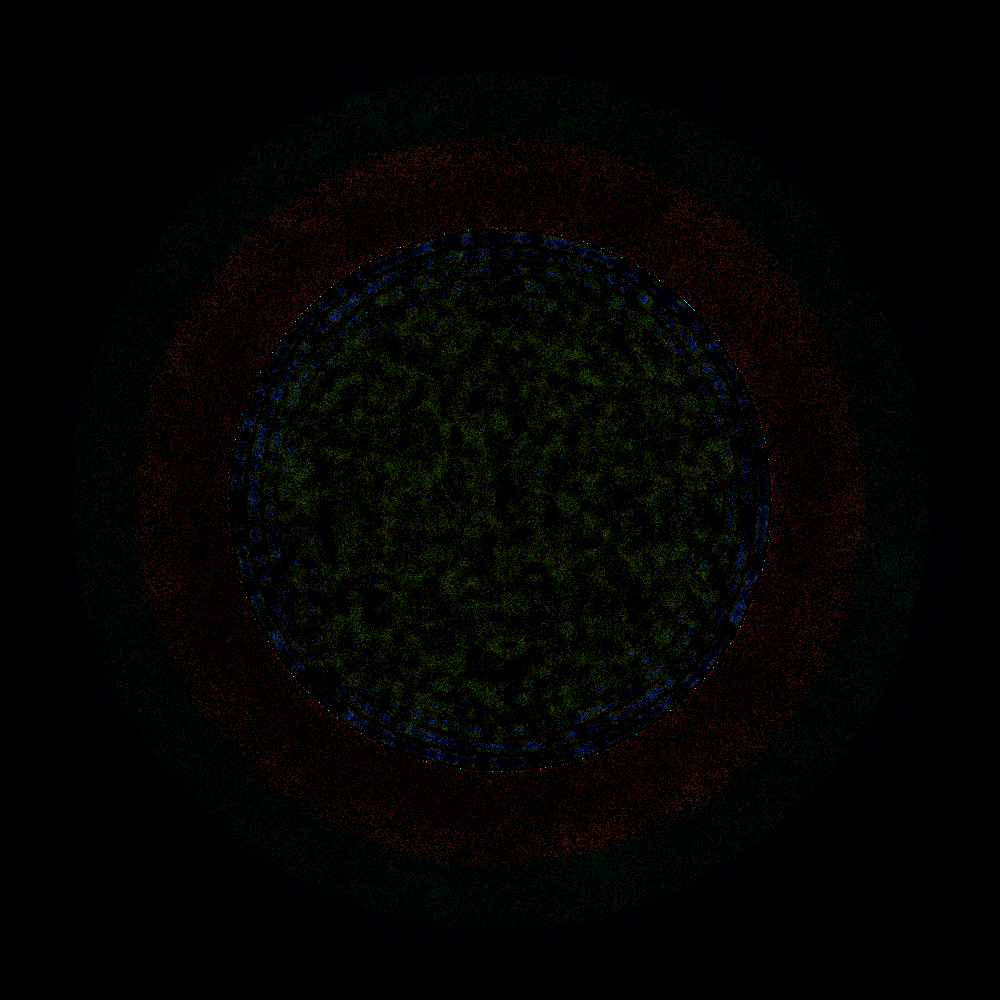
\includegraphics[width=0.6\linewidth]{figures/shuffle/diff-1234560}
\caption{An Image Generated by Subtracting \ref{fig:diff-1234560-rm} from \ref{fig:controlb}.}
\label{fig:diff-1234560}
\end{figure}

Figure \ref{fig:1234560} provides the thermal flux and fission rate meshes and geometric cross sections axially and radially.  Figure \ref{fig:diff-1234560} is the result of the image difference between the full core control mesh and Figure \ref{fig:1234560-rm}.

\begin{figure}[H]
\centering

\begin{subfigure}{0.45\textwidth}
  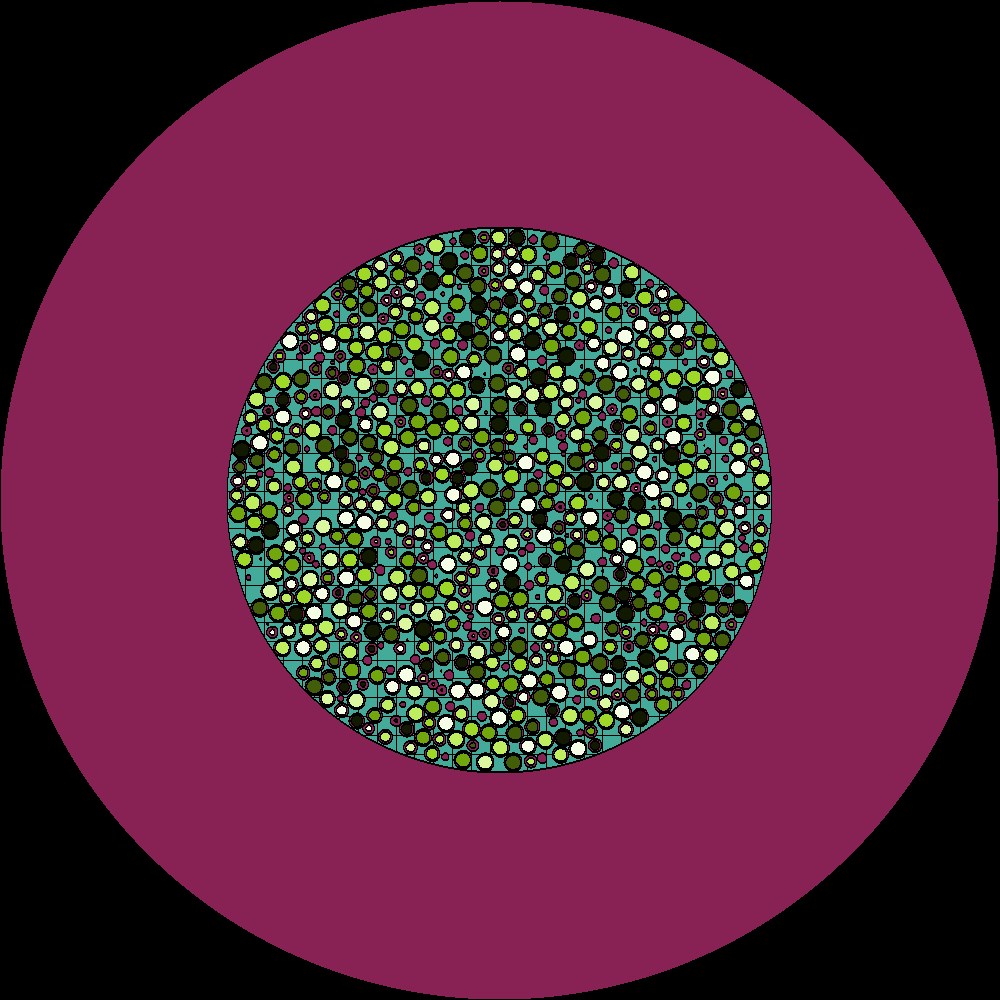
\includegraphics[width=0.95\linewidth]{figures/2345601/2345601-r}
  \caption{Radial Cross Section at y=0}
  \label{fig:2345601-r}
\end{subfigure}%
%
\begin{subfigure}{0.45\textwidth}
  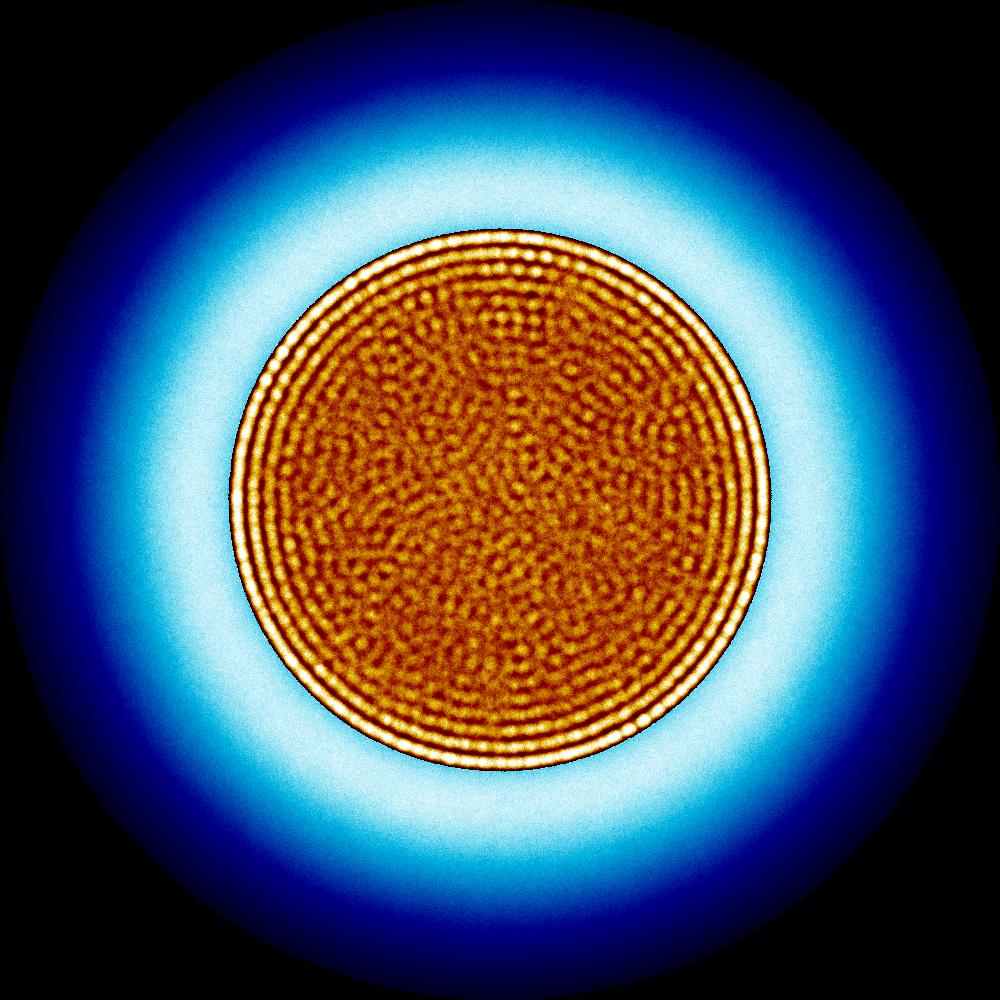
\includegraphics[width=0.95\linewidth]{figures/2345601/2345601-rm}
  \caption{Radial Mesh}
  \label{fig:2345601-rm}
\end{subfigure}

\begin{subfigure}{0.45\textwidth}
  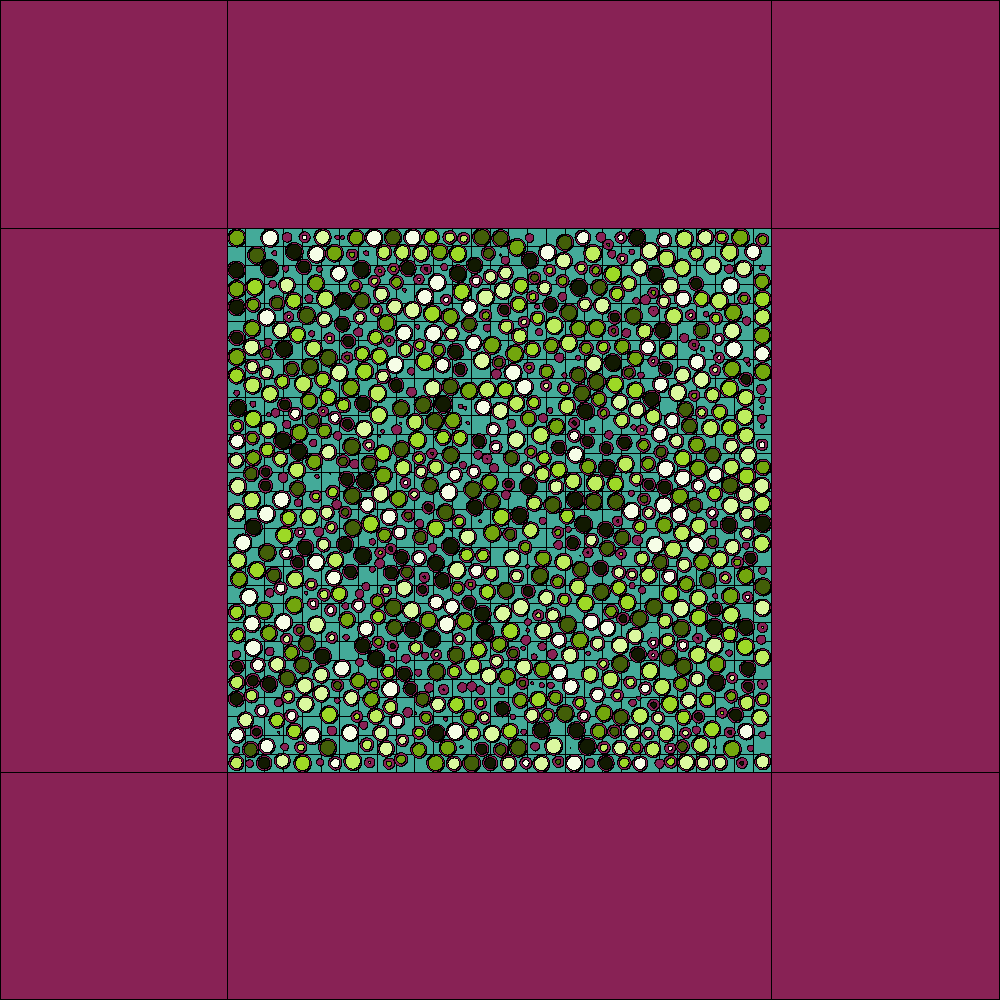
\includegraphics[width=0.95\linewidth]{figures/2345601/2345601-v}
  \caption{Axial Cross Section at z=0 }
  \label{fig:2345601-v}
\end{subfigure}
%
\begin{subfigure}{0.45\textwidth}
  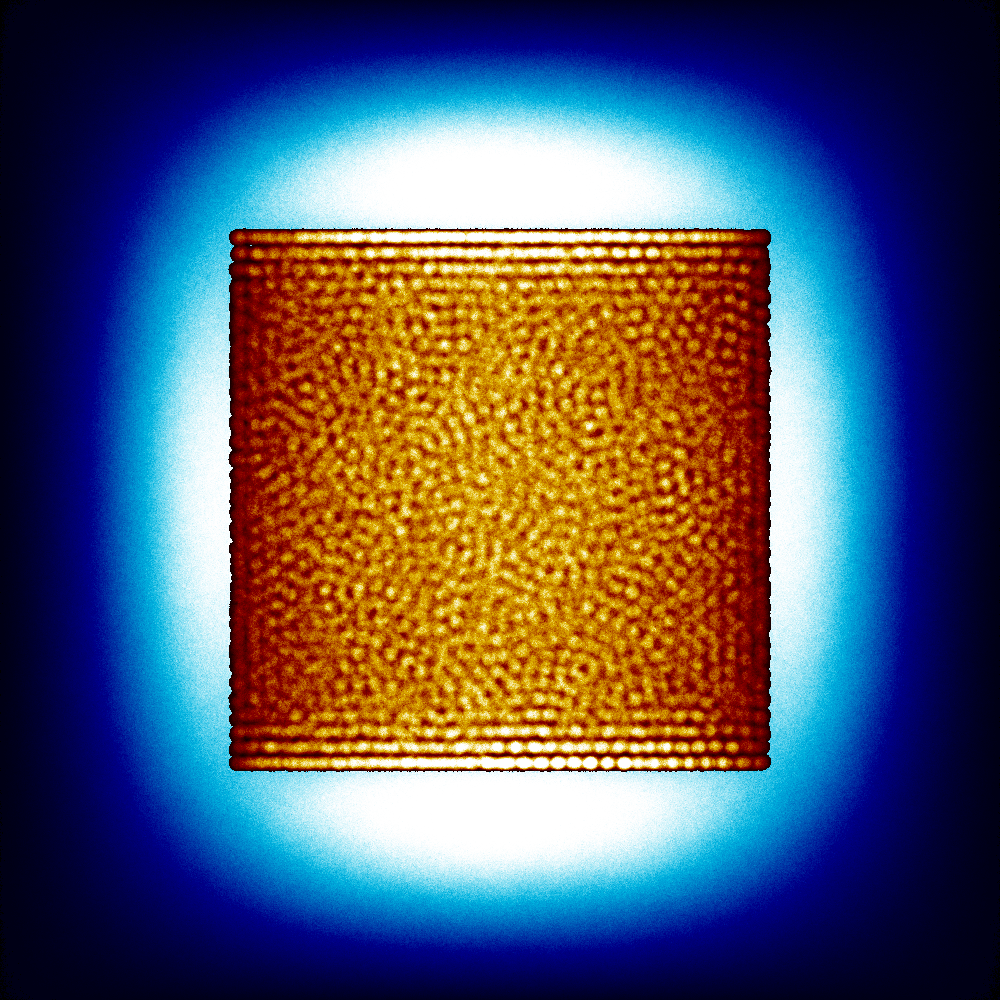
\includegraphics[width=0.95\linewidth]{figures/2345601/2345601-vm}
  \caption{Axial Mesh}
  \label{fig:2345601-vm}
\end{subfigure}
%
\caption{Shuffle Analysis: Run 2}
\label{fig:0-60}
\end{figure}
\begin{figure}[H]
\centering
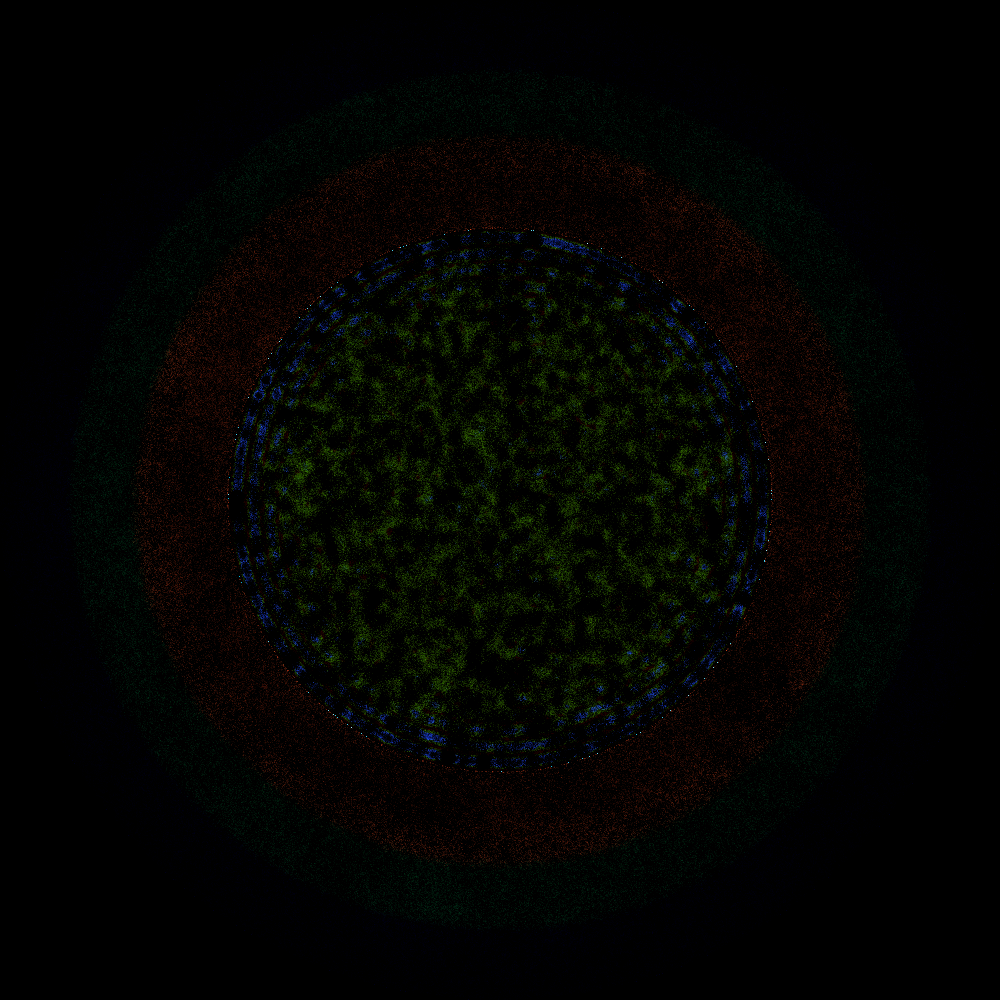
\includegraphics[width=0.6\linewidth]{figures/shuffle/diff-2345601}
\caption{An Image Generated by Subtracting \ref{fig:2345601-rm} from \ref{fig:controlb}.}
\label{fig:diff-2345601}
\end{figure}

Figure \ref{fig:2345601} provides the thermal flux and fission rate meshes and geometric cross sections axially and radially.  Figure \ref{fig:diff-2345601} is the result of the image difference between the full core control mesh and Figure \ref{fig:2345601-rm}.

\begin{figure}[H]
\centering

\begin{subfigure}{0.45\textwidth}
  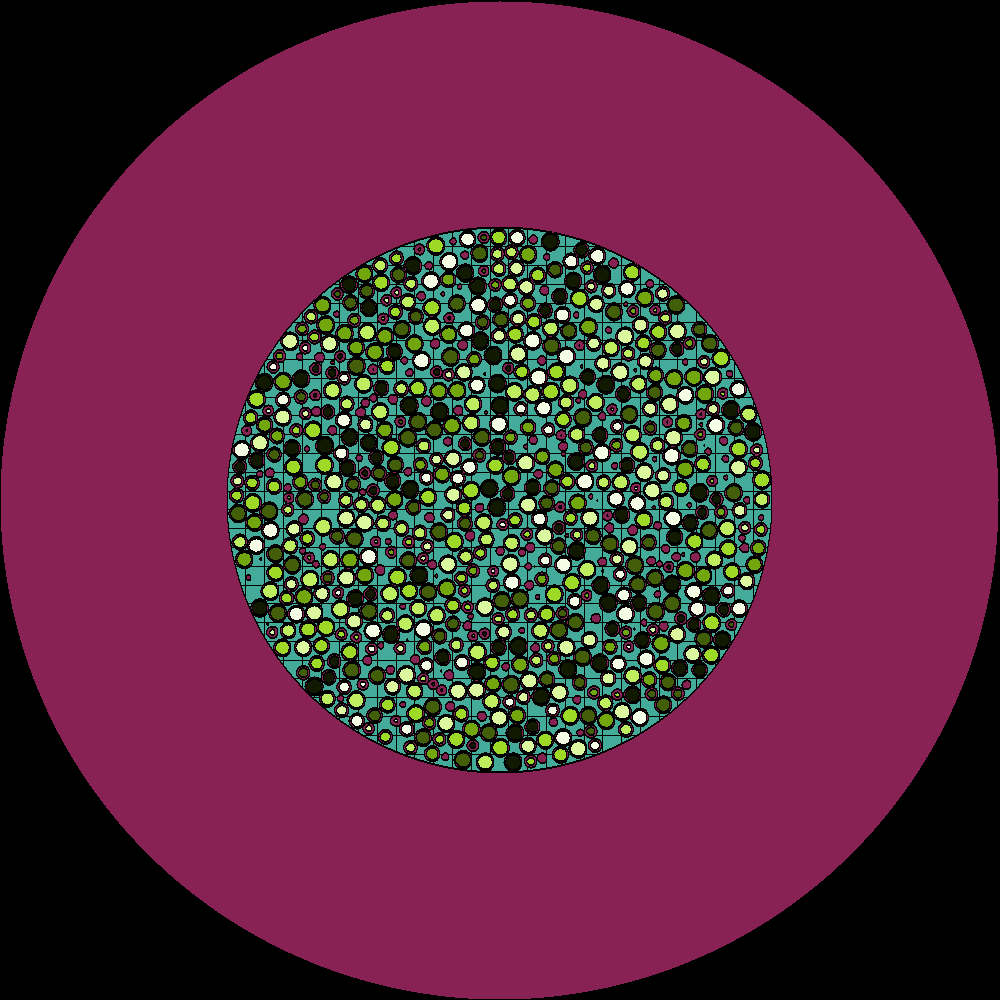
\includegraphics[width=0.95\linewidth]{figures/3456012/3456012-r}
  \caption{Radial Cross Section at y=0}
  \label{fig:3456012-r}
\end{subfigure}%
%
\begin{subfigure}{0.45\textwidth}
  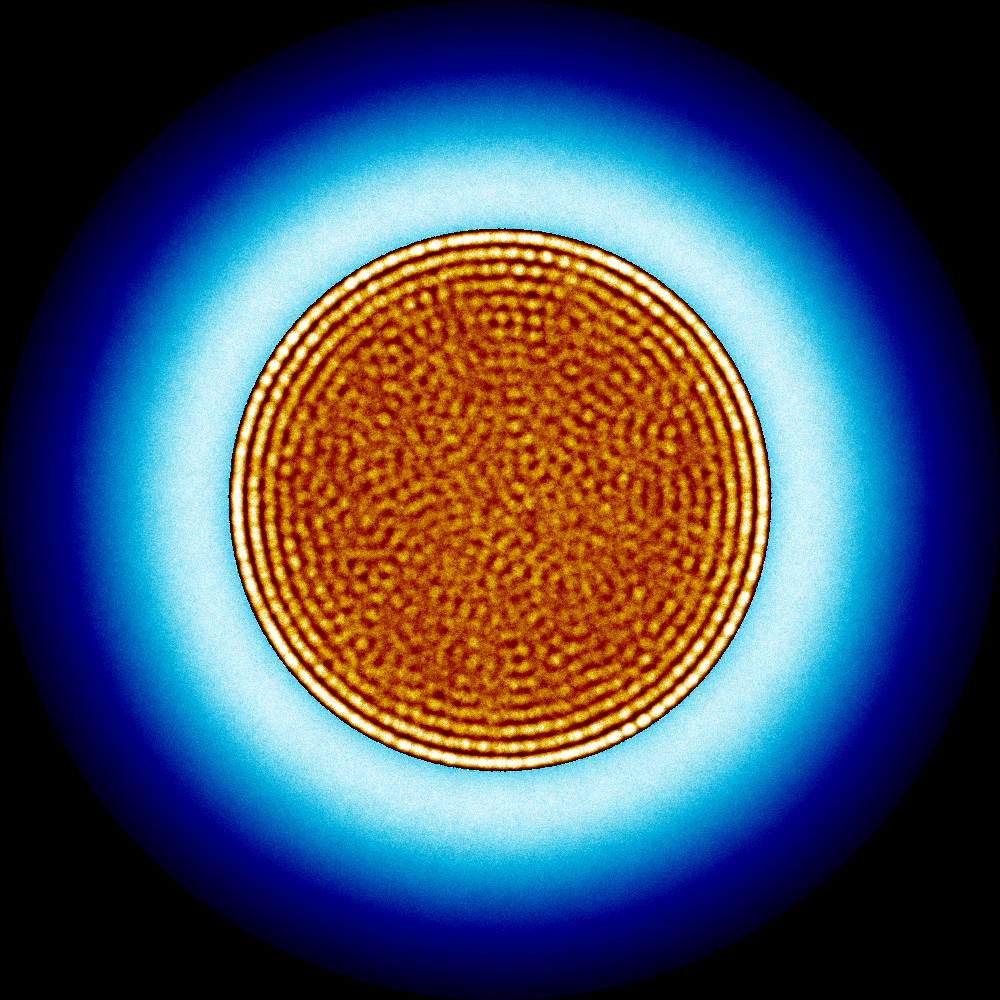
\includegraphics[width=0.95\linewidth]{figures/3456012/3456012-rm}
  \caption{Radial Mesh}
  \label{fig:3456012-rm}
\end{subfigure}

\begin{subfigure}{0.45\textwidth}
  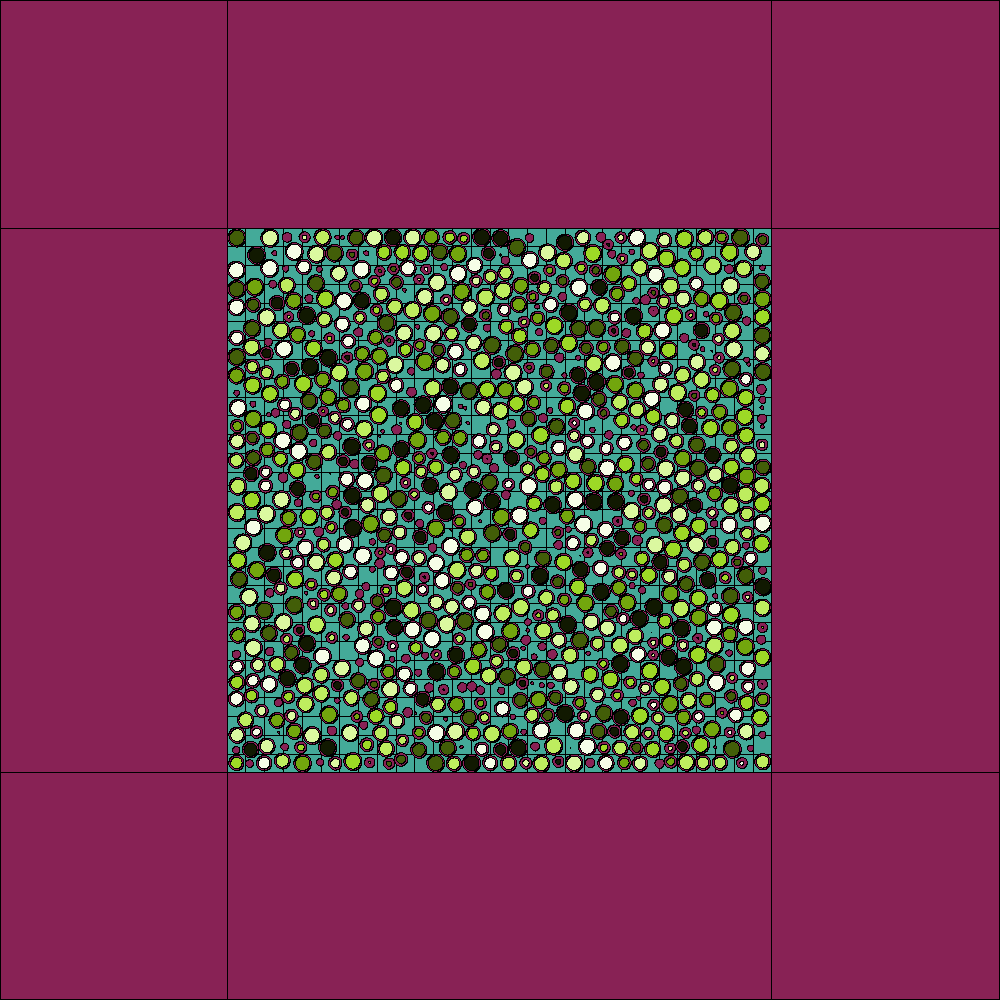
\includegraphics[width=0.95\linewidth]{figures/3456012/3456012-v}
  \caption{Axial Cross Section at z=0 }
  \label{fig:3456012-v}
\end{subfigure}
%
\begin{subfigure}{0.45\textwidth}
  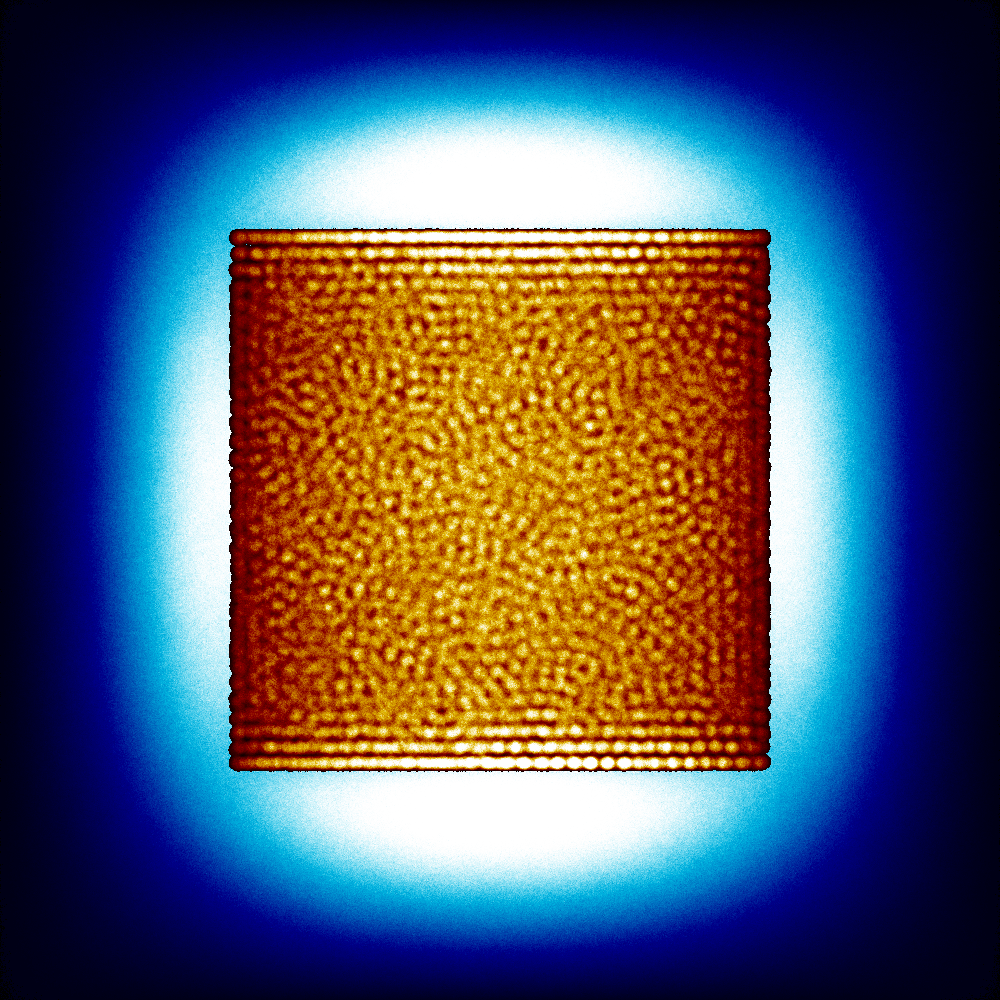
\includegraphics[width=0.95\linewidth]{figures/3456012/3456012-vm}
  \caption{Axial Mesh}
  \label{fig:3456012-vm}
\end{subfigure}
%
\caption{Shuffle Analysis: Run 3}
\label{fig:3456012}
\end{figure}
\begin{figure}[H]
\centering
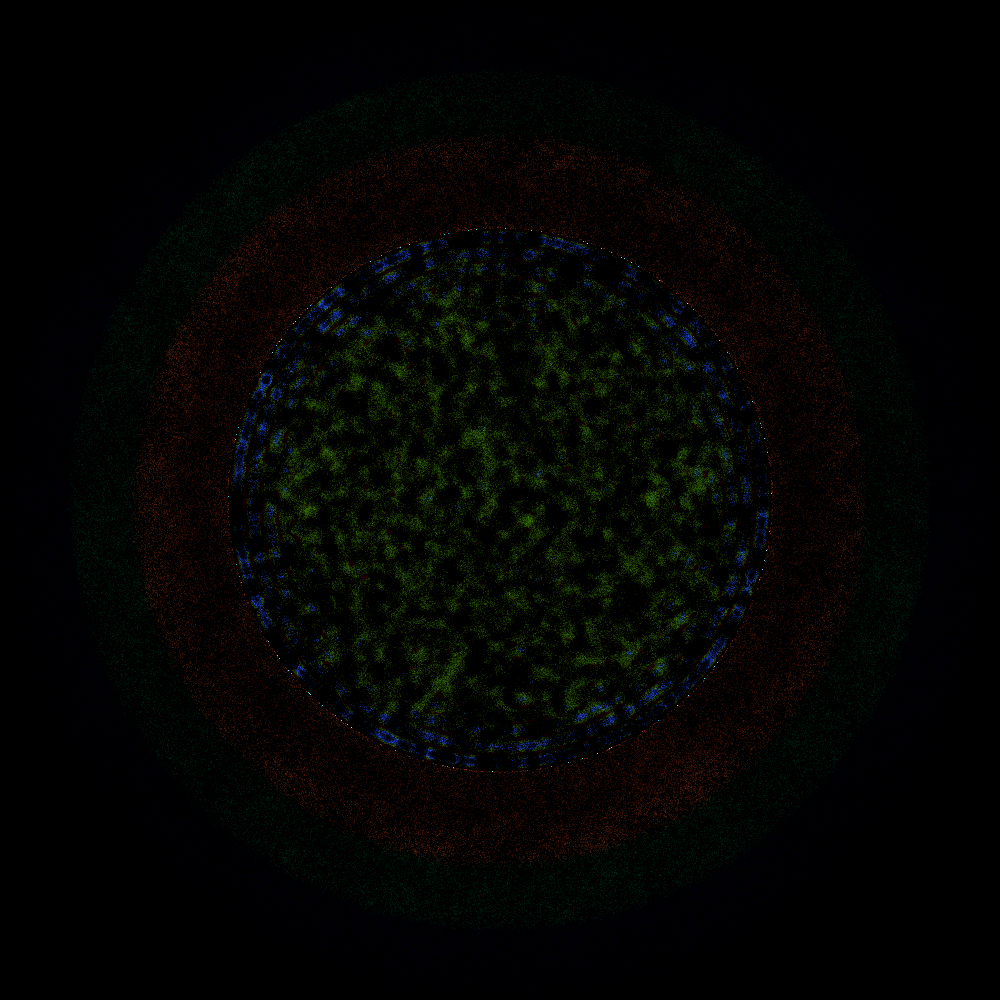
\includegraphics[width=0.6\linewidth]{figures/shuffle/diff-3456012}
\caption{An Image Generated by Subtracting Figure \ref{fig:3456012-rm} from Figure \ref{fig:controlb}.}
\label{fig:diff-3456012}
\end{figure}

Figure \ref{fig:3456012} provides the thermal flux and fission rate meshes and geometric cross sections axially and radially.  Figure \ref{fig:diff-3456012} is the result of the image difference between the full core control mesh and Figure \ref{fig:3456012-rm}.

\begin{figure}[H]
\centering

\begin{subfigure}{0.45\textwidth}
  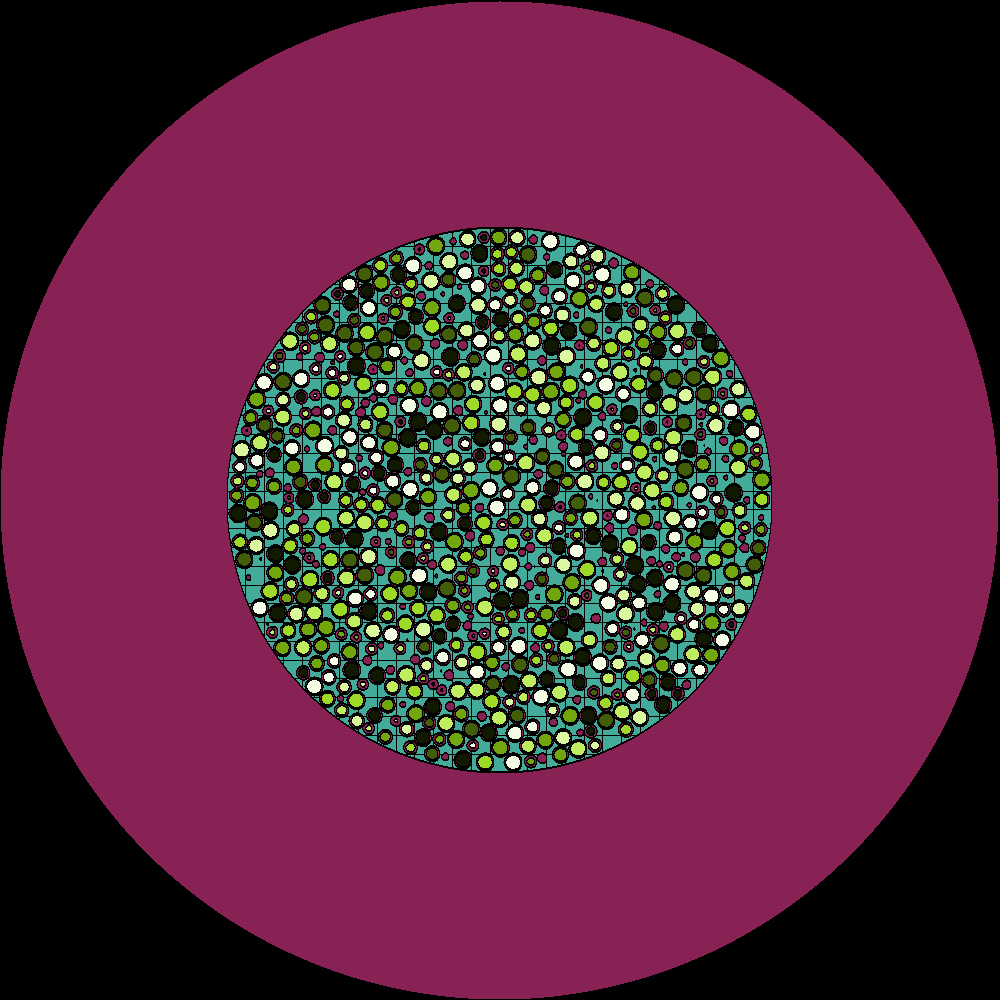
\includegraphics[width=0.95\linewidth]{figures/4560123/4560123-r}
  \caption{Radial Cross Section at y=0}
  \label{fig:4560123-r}
\end{subfigure}%
%
\begin{subfigure}{0.45\textwidth}
  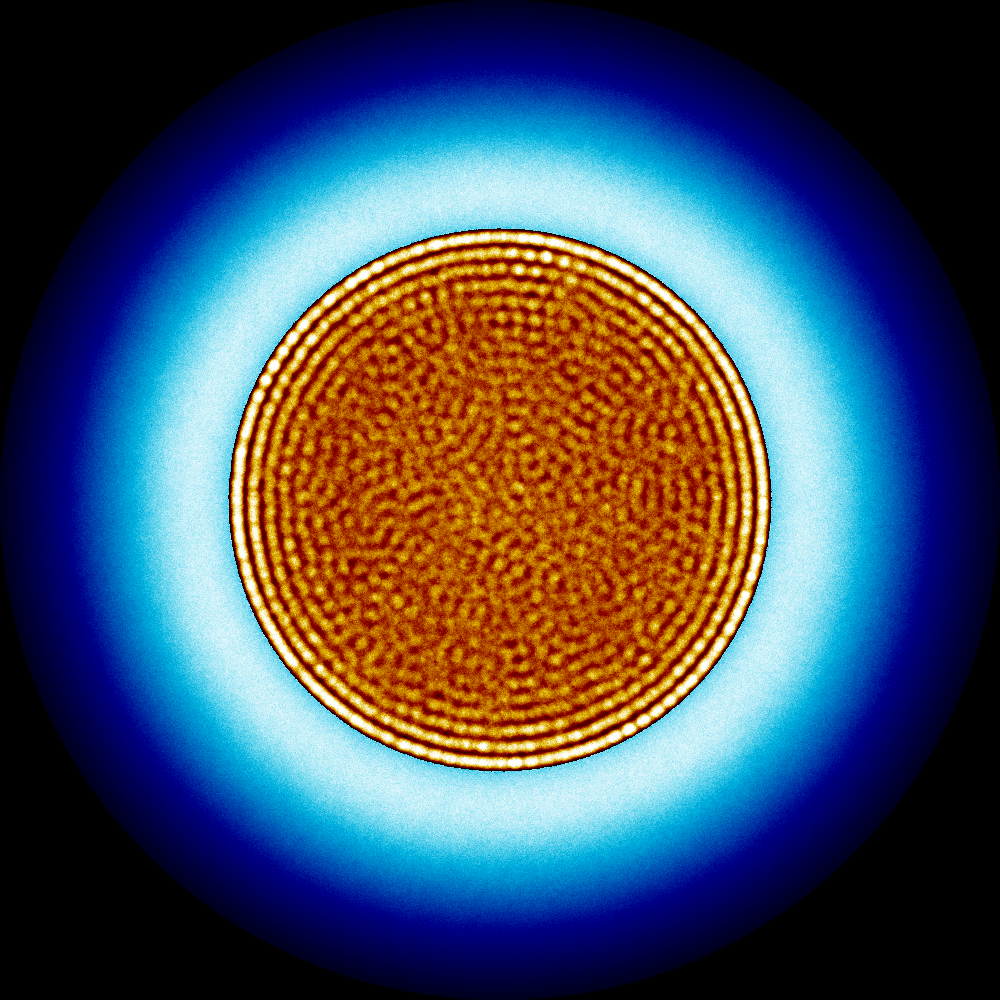
\includegraphics[width=0.95\linewidth]{figures/4560123/4560123-rm}
  \caption{Radial Mesh}
  \label{fig:4560123-rm}
\end{subfigure}

\begin{subfigure}{0.45\textwidth}
  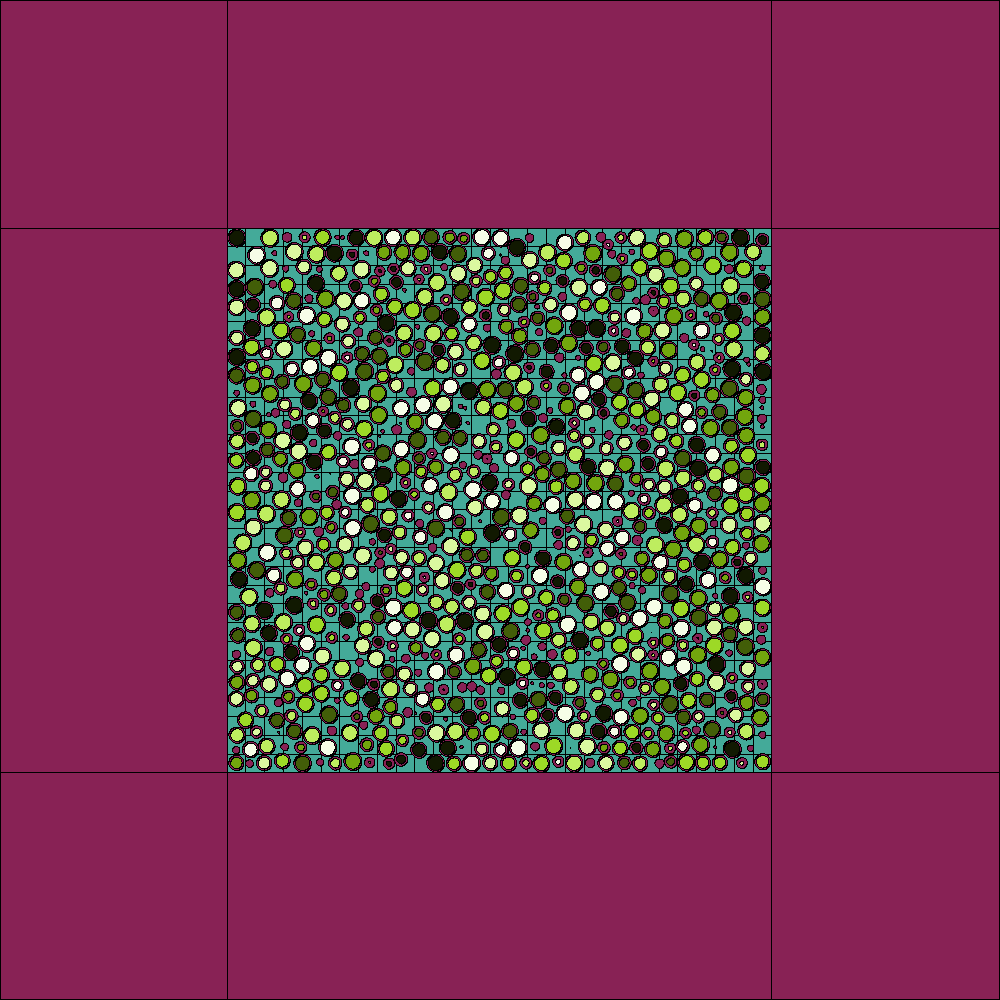
\includegraphics[width=0.95\linewidth]{figures/4560123/4560123-v}
  \caption{Axial Cross Section at z=0 }
  \label{fig:4560123-v}
\end{subfigure}
%
\begin{subfigure}{0.45\textwidth}
  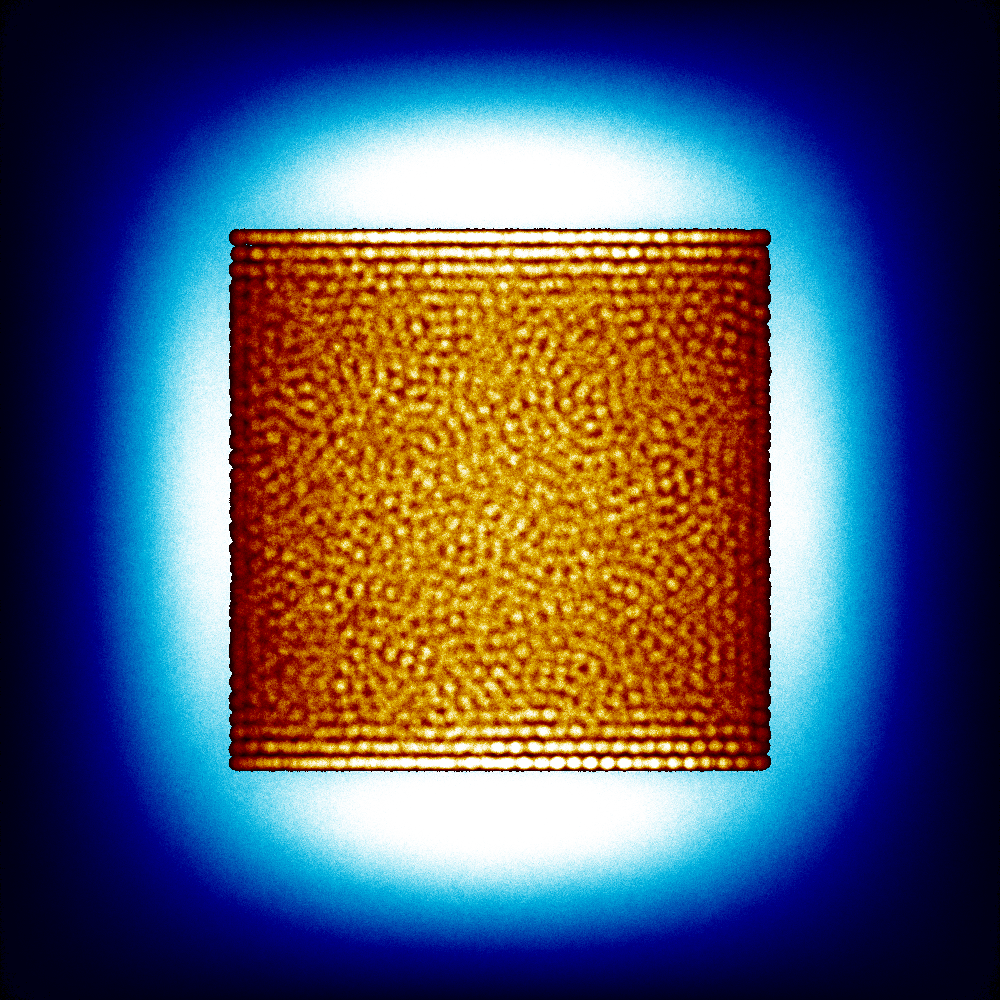
\includegraphics[width=0.95\linewidth]{figures/4560123/4560123-vm}
  \caption{Axial Mesh}
  \label{fig:4560123-vm}
\end{subfigure}
%
\caption{Shuffle Analysis: Run 4}
\label{fig:4560123}
\end{figure}
\begin{figure}[H]
\centering
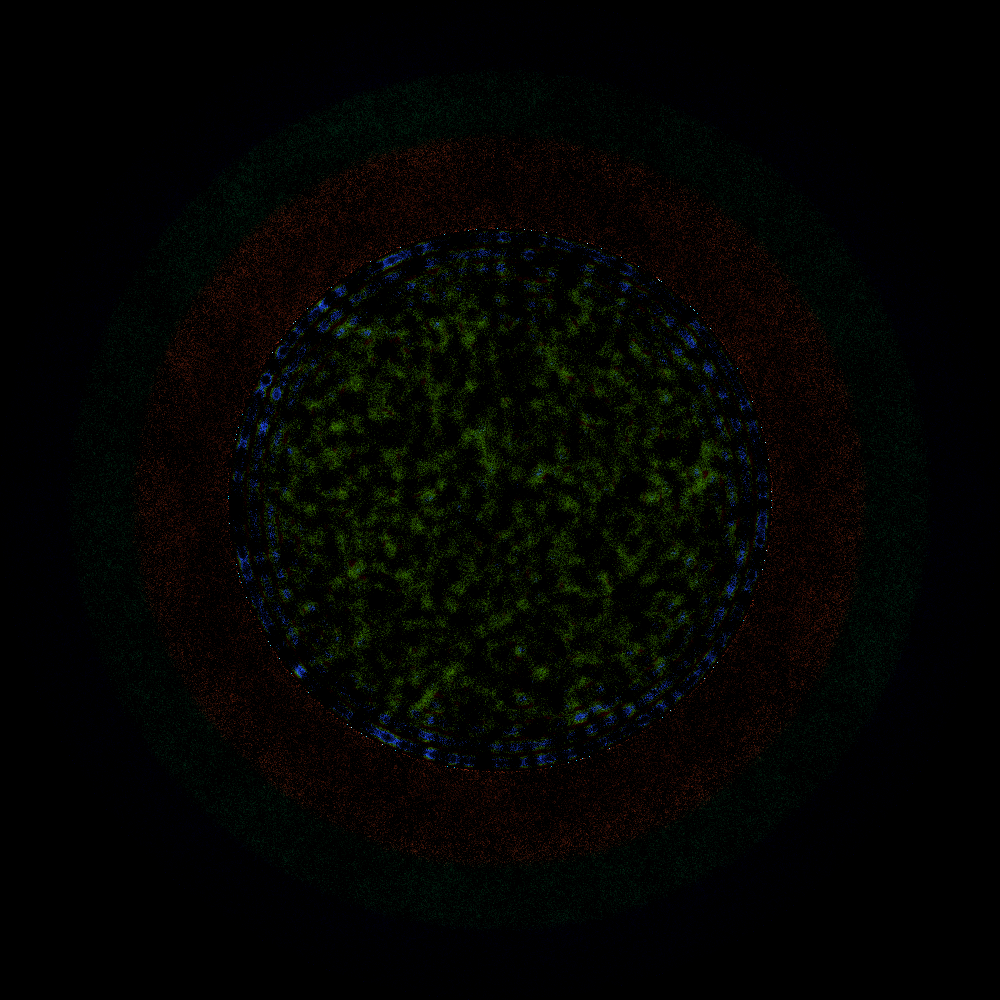
\includegraphics[width=0.6\linewidth]{figures/shuffle/diff-4560123}
\caption{An Image Generated by Subtracting \ref{fig:4560123-rm} from \ref{fig:controlb}.}
\label{fig:diff-4560123}
\end{figure}

Figure \ref{fig:4560123} provides the thermal flux and fission rate meshes and geometric cross sections axially and radially.  Figure \ref{fig:diff-4560123} is the result of the image difference between the full core control mesh and Figure \ref{fig:4560123-rm}.

\begin{figure}[H]
\centering

\begin{subfigure}{0.45\textwidth}
  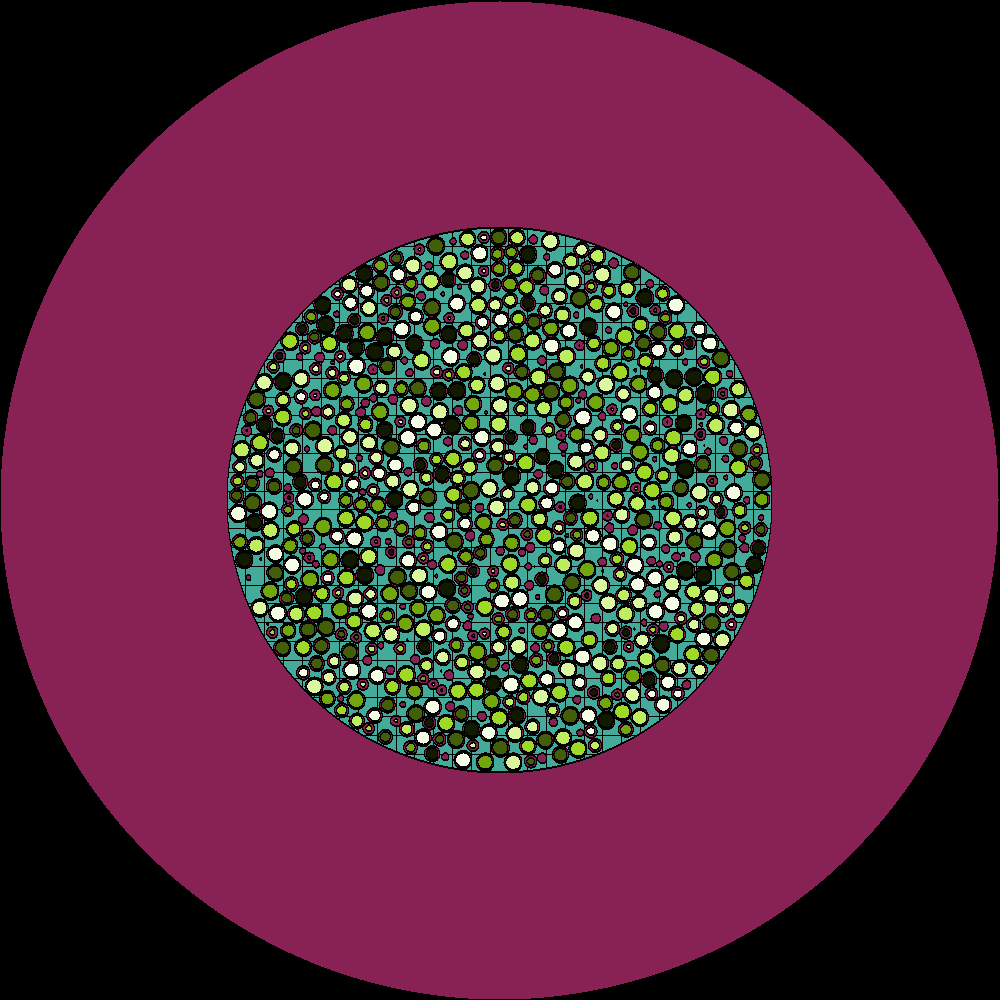
\includegraphics[width=0.95\linewidth]{figures/5601234/5601234-r}
  \caption{Radial Cross Section at y=0}
  \label{fig:5601234-r}
\end{subfigure}%
%
\begin{subfigure}{0.45\textwidth}
  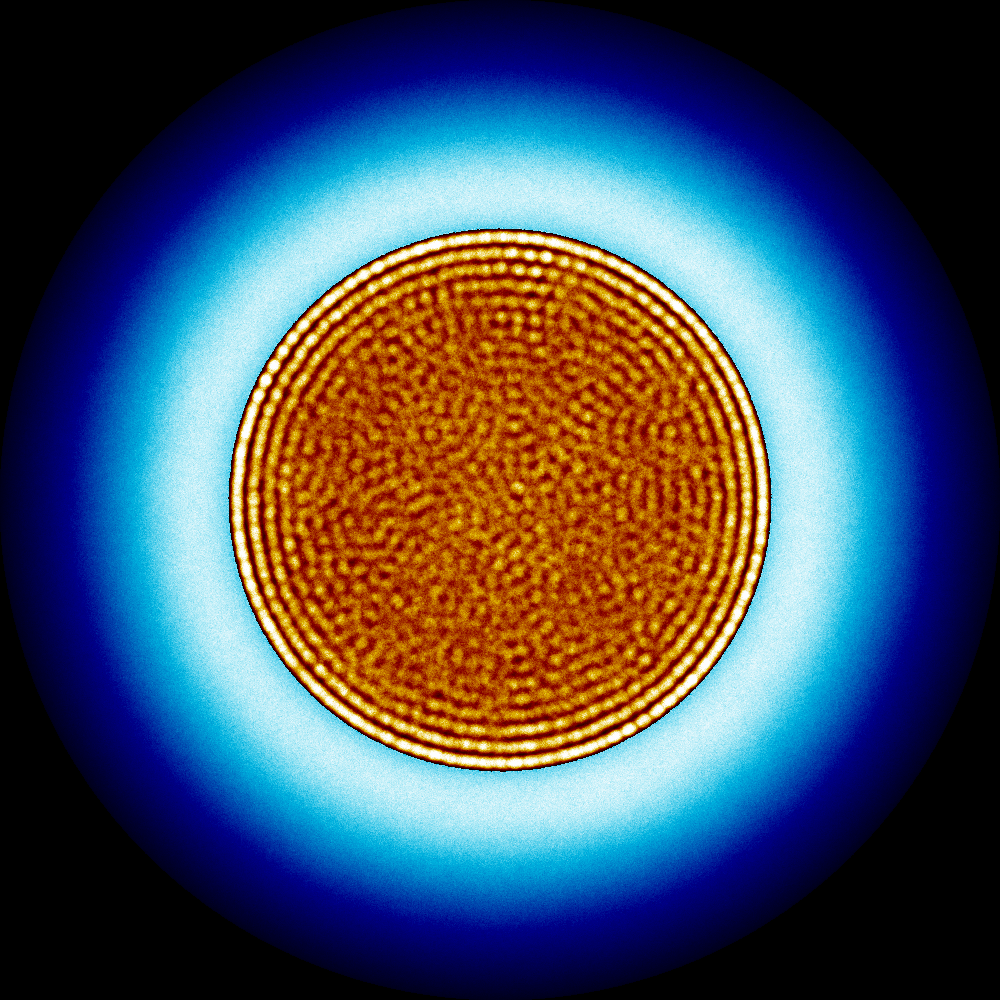
\includegraphics[width=0.95\linewidth]{figures/5601234/5601234-rm}
  \caption{Radial Mesh}
  \label{fig:5601234-rm}
\end{subfigure}

\begin{subfigure}{0.45\textwidth}
  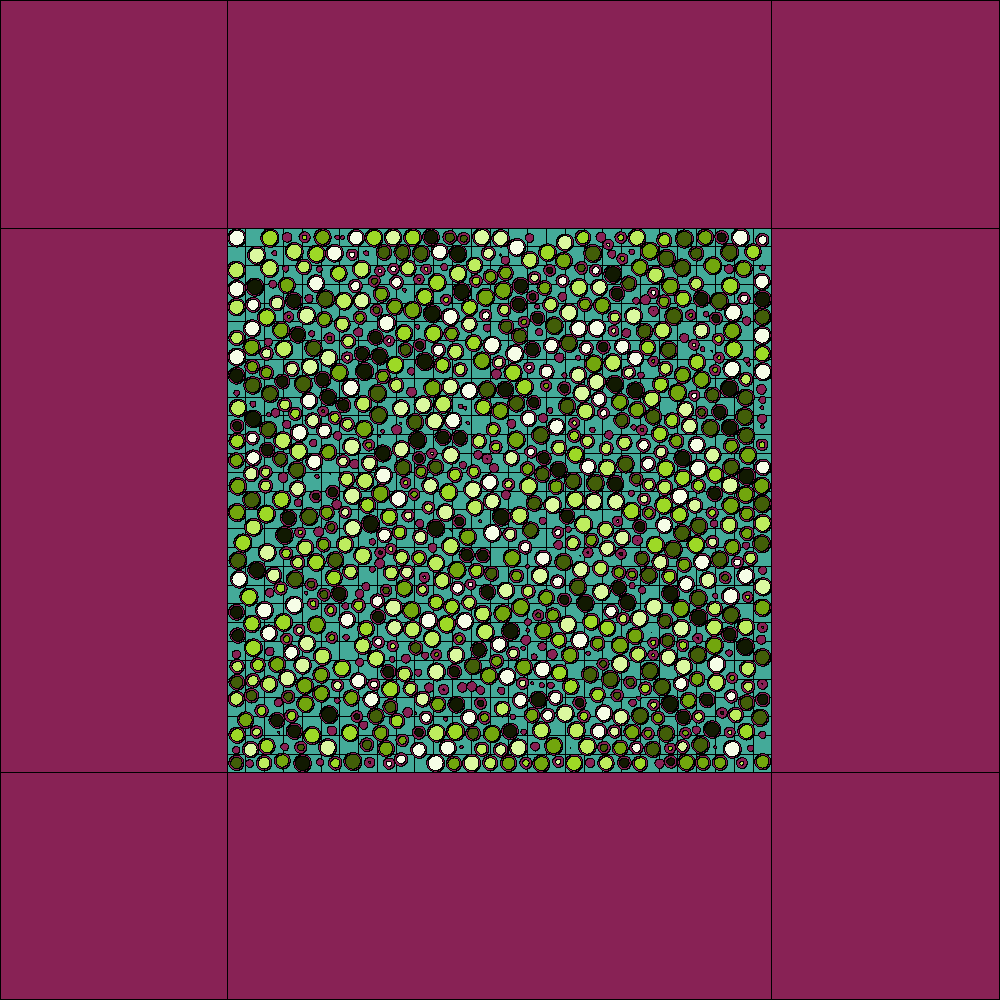
\includegraphics[width=0.95\linewidth]{figures/5601234/5601234-v}
  \caption{Axial Cross Section at z=0 }
  \label{fig:5601234-v}
\end{subfigure}
%
\begin{subfigure}{0.45\textwidth}
  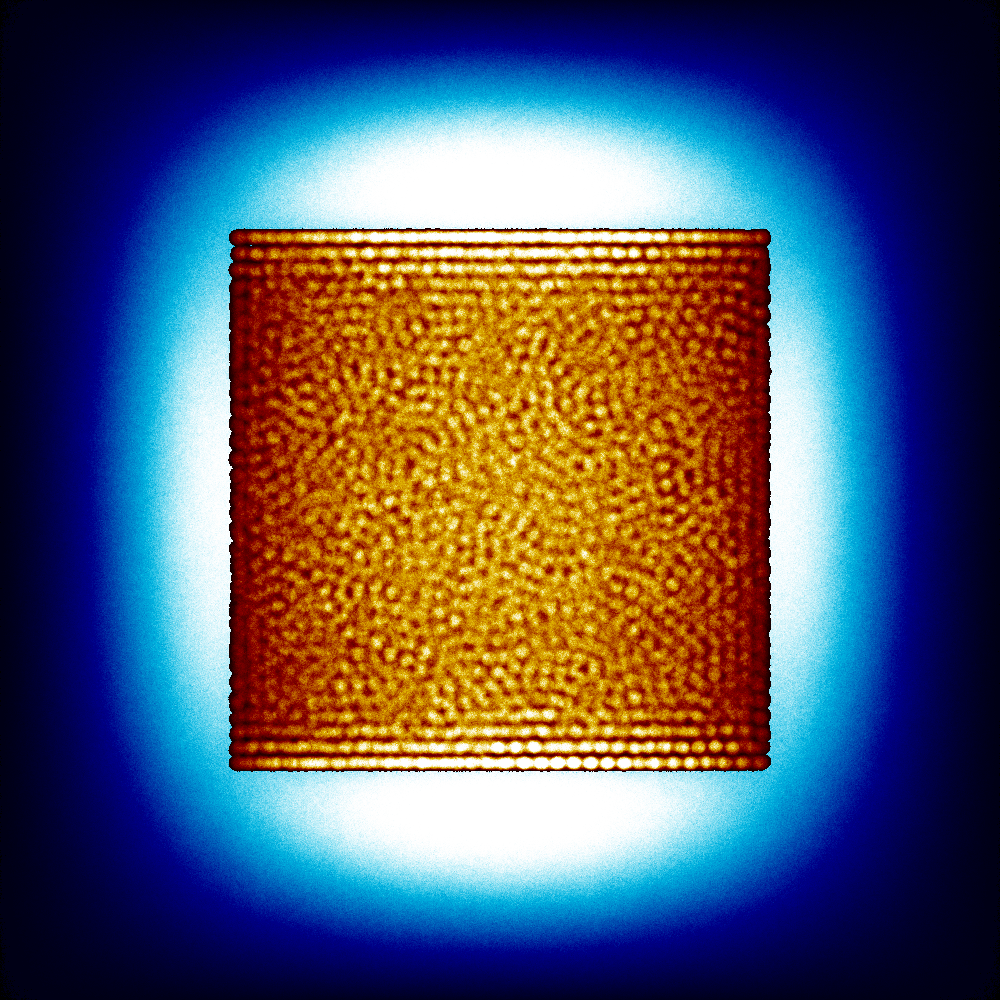
\includegraphics[width=0.95\linewidth]{figures/5601234/5601234-vm}
  \caption{Axial Mesh}
  \label{fig:5601234-vm}
\end{subfigure}
%
\caption{Shuffle Analysis: Run 5}
\label{fig:5601234}
\end{figure}
\begin{figure}[H]
\centering
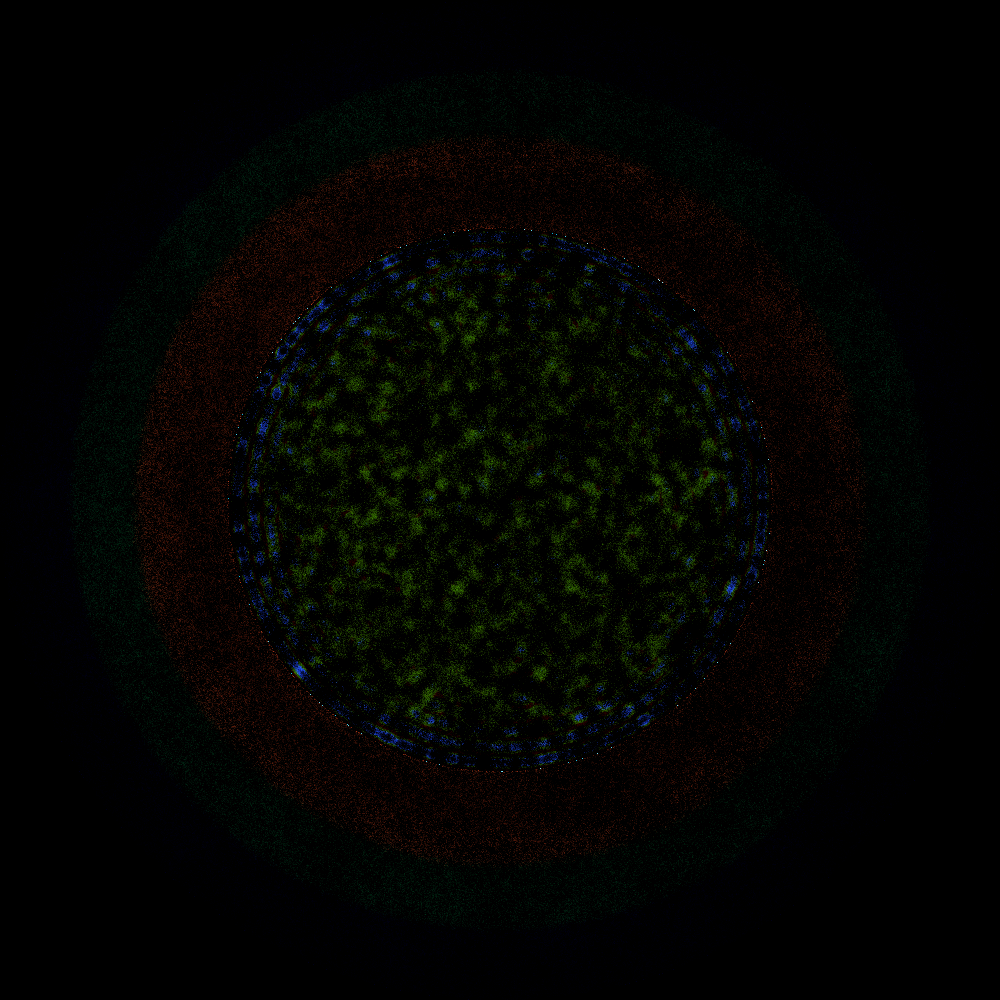
\includegraphics[width=0.6\linewidth]{figures/shuffle/diff-5601234}
\caption{An Image Generated by Subtracting \ref{fig:diff-5601234-rm} from \ref{fig:controlb}.}
\label{fig:diff-5601234}
\end{figure}

Figure \ref{fig:5601234} provides the thermal flux and fission rate meshes and geometric cross sections axially and radially.  Figure \ref{fig:diff-5601234} is the result of the image difference between the full core control mesh and Figure \ref{fig:5601234-rm}.

\begin{figure}[H]
\centering

\begin{subfigure}{0.45\textwidth}
  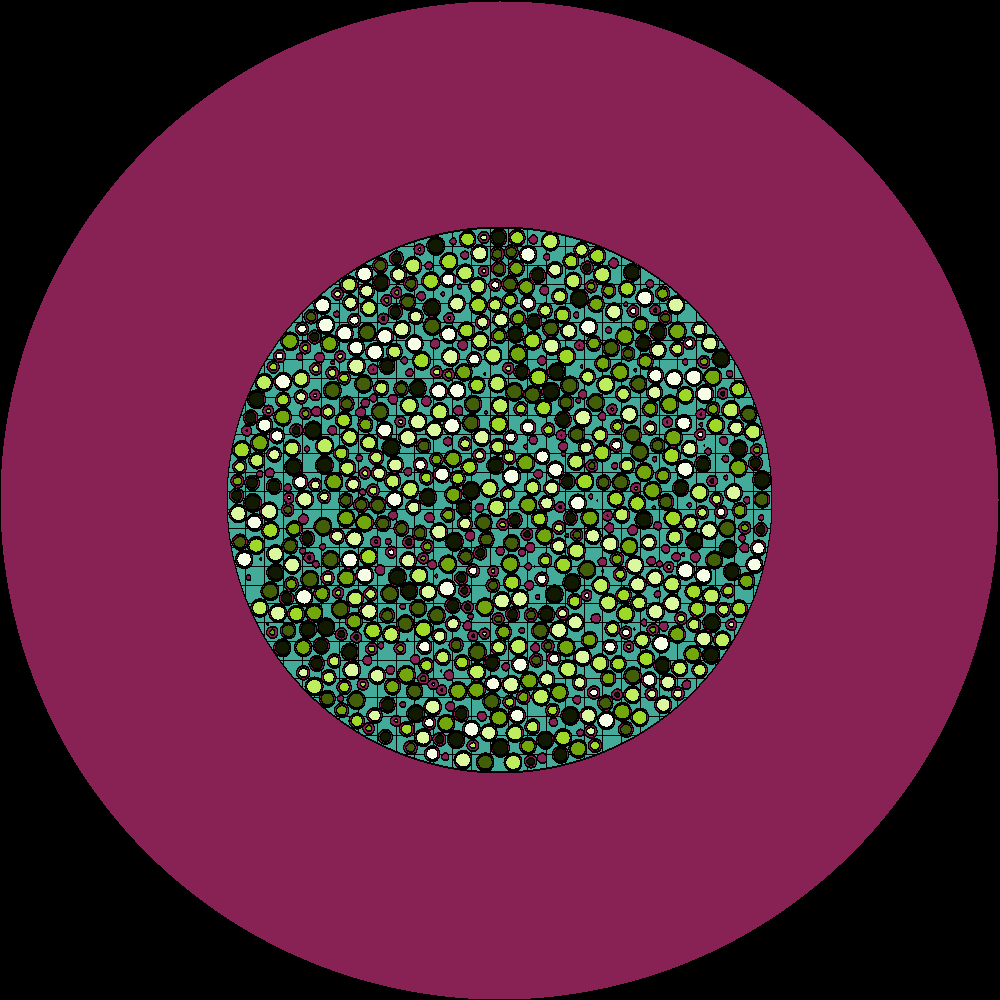
\includegraphics[width=0.95\linewidth]{figures/6012345/6012345-r}
  \caption{Radial Cross Section at y=0}
  \label{fig:6012345-r}
\end{subfigure}%
%
\begin{subfigure}{0.45\textwidth}
  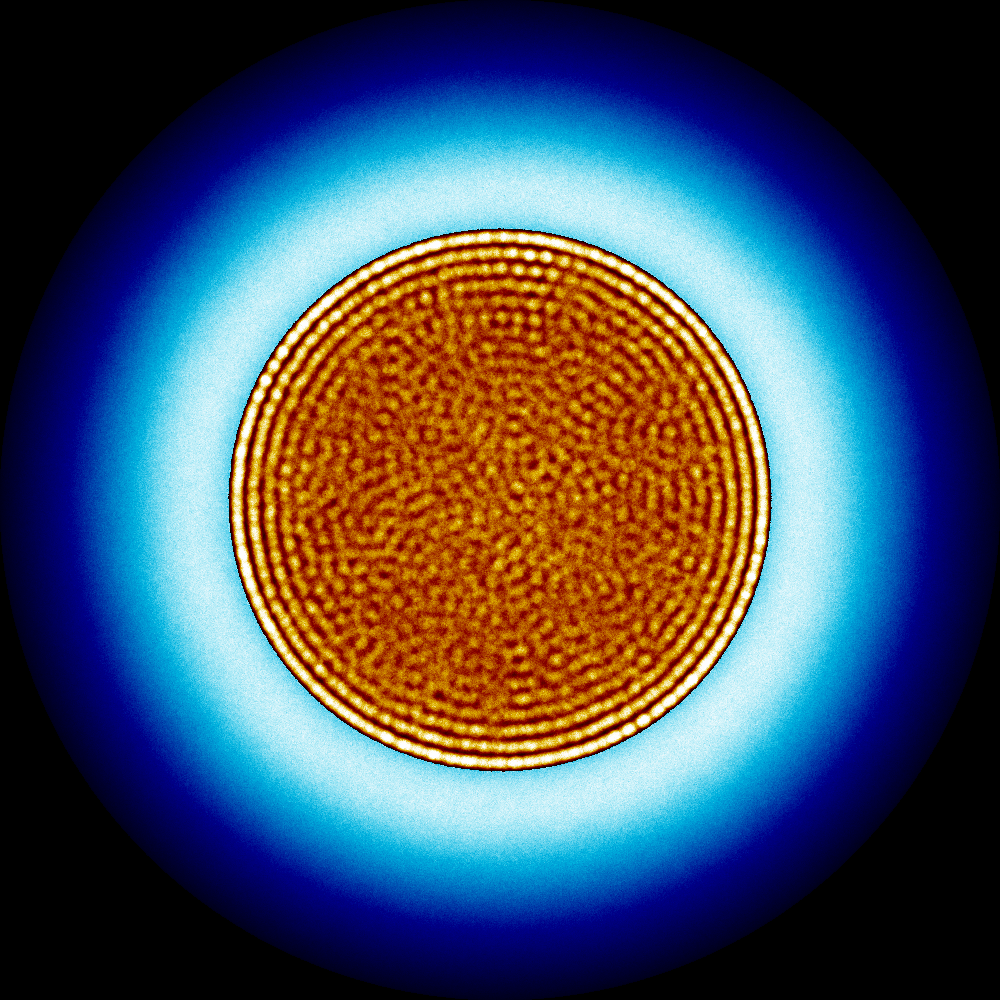
\includegraphics[width=0.95\linewidth]{figures/6012345/6012345-rm}
  \caption{Radial Mesh}
  \label{fig:6012345-rm}
\end{subfigure}

\begin{subfigure}{0.45\textwidth}
  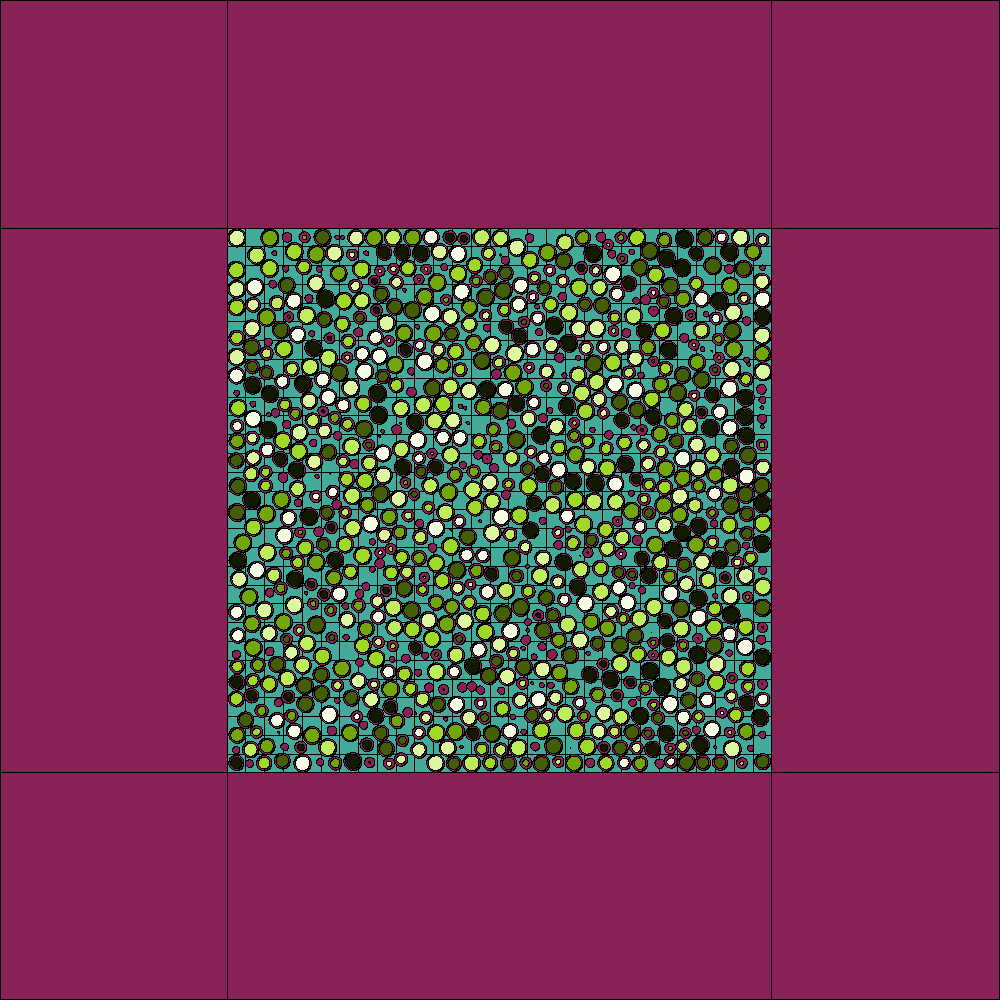
\includegraphics[width=0.95\linewidth]{figures/6012345/6012345-v}
  \caption{Axial Cross Section at z=0 }
  \label{fig:6012345-v}
\end{subfigure}
%
\begin{subfigure}{0.45\textwidth}
  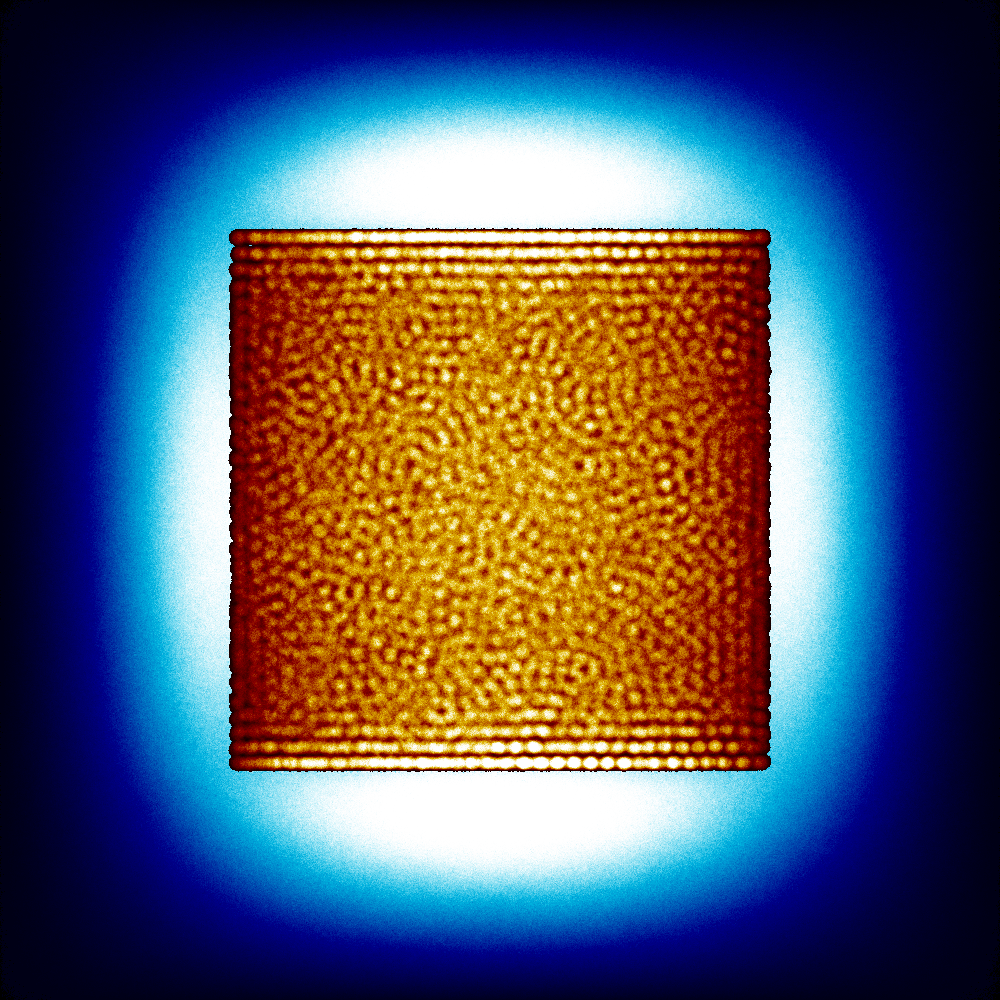
\includegraphics[width=0.95\linewidth]{figures/6012345/6012345-vm}
  \caption{Axial Mesh}
  \label{fig:6012345-vm}
\end{subfigure}
%
\caption{Shuffle Analysis: Run 6}
\label{fig:6012345}
\end{figure}
\begin{figure}[H]
\centering
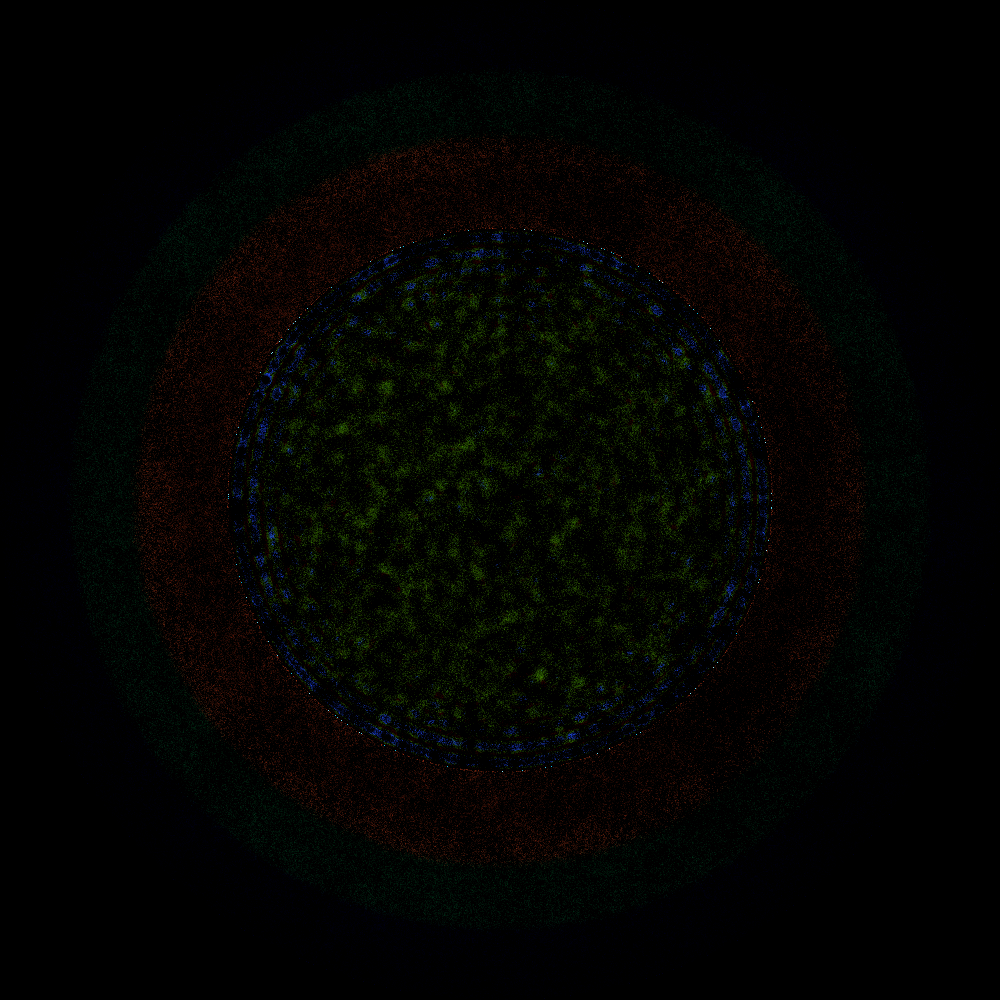
\includegraphics[width=0.6\linewidth]{figures/shuffle/diff-6012345}
\caption{An Image Generated by Subtracting Figure \ref{fig:6012345-rm} from Figure \ref{fig:controlb}.}
\label{fig:diff-6012345}
\end{figure}

Figure \ref{fig:6012345} provides the thermal flux and fission rate meshes and geometric cross sections axially and radially.  Figure \ref{fig:diff-6012345} is the result of the image difference between the full core control mesh and Figure \ref{fig:6012345-rm}.

There are a few hotspots where small regions show a brighter patch of green.  The best example of this is in the fourth quadrant of Figure \ref{fig:diff-6012345}, near the $270^{\circ}$ line.  Hotspots such as this could be caused by poor mixing, which would make some pebbles occur in higher concentrations (and then cause a larger difference in the shuffle test, when the same region is now dominated by a different burnup) or by the shuffling putting a different pebble burnup in a region of lower or higher flux.  To investigate the source of this, the pebbles in a ~10 cm square column (10 cm in x and y, the height of the reactor in z) around the hotspot were found.  Table \ref{table:10cmpebb} shows the count of each pebble burnup.


\begin{table}[H]
\centering
\caption{Representation of Pebbles by Number of Passes in a 10 cm Square Rectangular Prism Surrounding an Image Difference Hotspot at Approximately x = 11 cm, y = -56 cm}
 \begin{tabularx}{0.35\textwidth}{c  c}
 	\hline
 	Pebble Pass & Number of Pebbles \\
 	\hline
 	Fresh & 20 \\
 	First Pass & 12 \\
 	Second Pass & 13 \\
 	Third Pass & 12 \\
 	Fourth Pass & 10 \\
 	Fifth Pass & 14 \\
 	Sixth Pass & 11 \\
 	\hline
 \end{tabularx}
\label{table:10cmpebb}
\end{table}

When this region was narrowed further, to a ~5 cm region, the poor mixing was more dramatic, as seen in Table \ref{table:5cmpebb}.


\begin{table}[H]
\centering
\caption{Representation of Pebbles by Number of Passes in a 5 cm Square Rectangular Prism Surrounding an Image Difference Hotspot at Approximately x = 11 cm, y = -56 cm}
 \begin{tabularx}{0.35\textwidth}{c  c}
 	\hline
 	Pebble Pass & Number of Pebbles \\
 	\hline
 	Fresh & 10\\
 	First Pass & 3 \\
 	Second Pass & 4 \\
 	Third Pass & 1 \\
 	Fourth Pass & 2 \\
 	Fifth Pass & 2 \\
 	Sixth Pass & 2 \\
 	\hline

 \end{tabularx}
\label{table:5cmpebb}
\end{table}

In the 10 cm square column, fresh pebbles originally make up 21.7\% of all pebbles in the region.  In the 5cm square column that is tighter around the hotspot, fresh pebbles make up 41.7\% of all pebbles.  The hotspot pointed out in Figure \ref{fig:diff-6012345} exists in some degree in Figures \ref{fig:diff-1234560}, \ref{fig:diff-2345601}, \ref{fig:diff-3456012}, \ref{fig:diff-4560123}, and \ref{fig:diff-5601234} --- it is simply brightest in Figure \ref{fig:diff-6012345} because the shuffle scheme corresponding to this Figure \ref{fig:diff-6012345} replaces fresh pebbles with 6-pass pebbles, which have the greatest disparity in burnup.